\appendix
\chapter{Development}
\label{chap:app_dev}

The setup uses the libraries presented in section \ref{sec:app_libs}. The tf-agents library has to be adjusted, to be able to use action-masking with PPO agents. The code for the value network is missing an argument to determine, whether to use a mask, or not. Therefore, a new argument has to be added. The file is located under \verb|/usr/local/lib/python3.8/dist-packages/tf_agents/networks/value_network.py|. The argument \verb|mask=None| has to be added to the function \verb|call| for action-masking to work. An issue (\#762) addressing this problem was created in the tf-agent repository on Github, but as of 29.11.2022 no reply.

The whole setup process can be done automatically with \textit{Docker} on a Windows operation system. The scripts, \ref{sec:app_batch} and \ref{sec:app_docker}, have to be saved in the same folder with their respective names. In addition to making the previously mentioned code modifications, all necessary libraries will be installed in a Linux container, by executing \textit{start.bat}. Finally, the container will be started and will listen to multiple ports, so statistics can be presented via \textit{Tensorboard} hosted on localhost.

\section{Libraries}
\label{sec:app_libs}

Following libraries and versions were used for the setup:

\begin{itemize}
	
	\item{Docker desktop: 4.11.1}
	\item{Python: 3.8.10}
		\begin{itemize}
			\item{IPython: 8.3.0}
			\item{ipykernel: 5.1.1}
			\item{tf-agents: 0.13.0}
			\item{dm-reverb: 0.8.0}
		\end{itemize}

\end{itemize}


\section{start.bat}
\label{sec:app_batch}


\begin{verbatim}
docker build -t rl/tf_agents_with_reverb:2.9.1 .
docker run --name tfagents-reverb -p 8888:8888 -p 6006-6009:6006-6009 rl/tf_agents_with_reverb:2.9.1
\end{verbatim}

\section{Dockerfile}
\label{sec:app_docker}

\begin{verbatim}
FROM tensorflow/tensorflow:2.9.1-jupyter

RUN pip install tf-agents==0.13.0
RUN pip install dm-reverb==0.8.0

# https://github.com/tensorflow/agents/issues/762
RUN sed -i 's/training=False/training=False, mask=None/g' /usr/local/lib/python3.8/dist-packages/tf_agents/networks/value_network.py

WORKDIR "/tf"
RUN rm -rf tensorflow-tutorials
COPY ./ /tf/
\end{verbatim}

\chapter{Experiments}
\label{chap:app_exp}


\section{DDQN}

\begin{figure}[H]
	\centering
	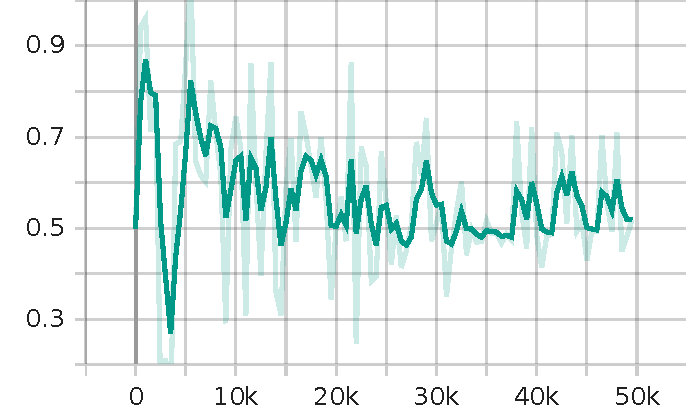
\includegraphics[scale=.75]{images/stats/ddqn_50k/Losses_td_loss}
	\caption[DDQN loss]{Loss of the DDQN agent in Mastermind. The x-axis displays the number of training steps and the y-axis the loss value.}
	\label{fig:ddqn_tderr}
\end{figure}

Initially, in contrast to the remaining values, the DDQN agent is having high extremes, 0.87 as its highest and 0.27 as its lowest value for the loss. However, after training for 10.000 steps it is starting to stabilize and not having that high spikes again, as seen in figure \ref{fig:ddqn_tderr}.

\begin{figure}[H]
	\centering
	\subfloat[Training: Average episode length]{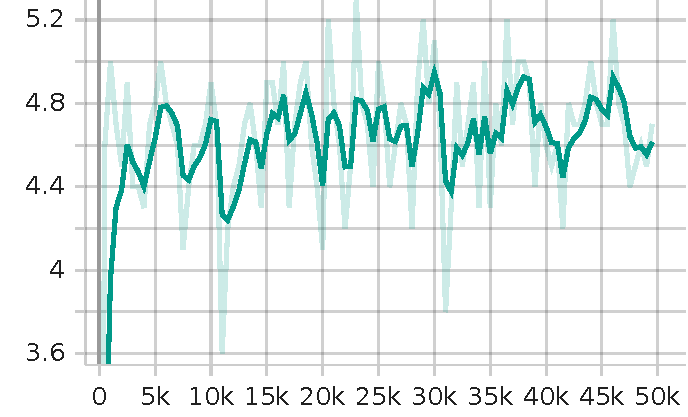
\includegraphics[scale=.6]{images/stats/ddqn_50k/Metrics_Train_AverageEpisodeLength} }
	\qquad
	\subfloat[Training: Average return]{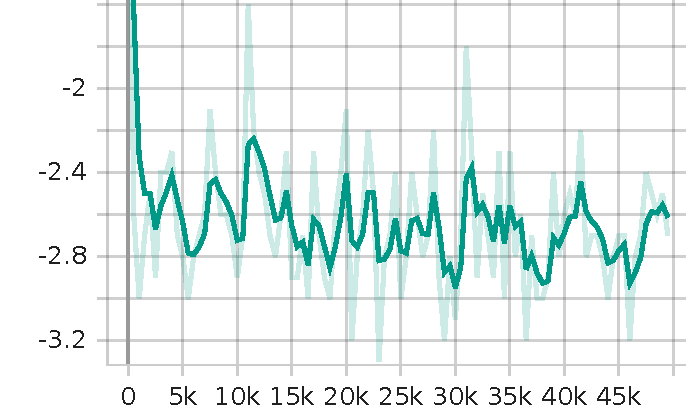
\includegraphics[scale=.6]{images/stats/ddqn_50k/Metrics_Train_AverageReturn} }
	\qquad
	\subfloat[Evaluation: Average episode length]{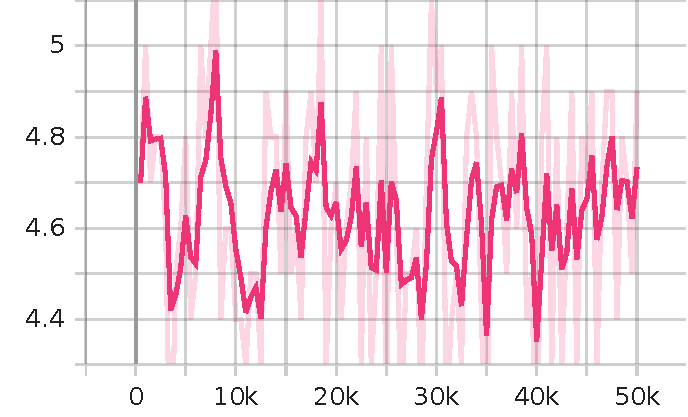
\includegraphics[scale=.6]{images/stats/ddqn_50k/Metrics_Eval_AverageEpisodeLength} }
	\qquad
	\subfloat[Evaluation: Average return]{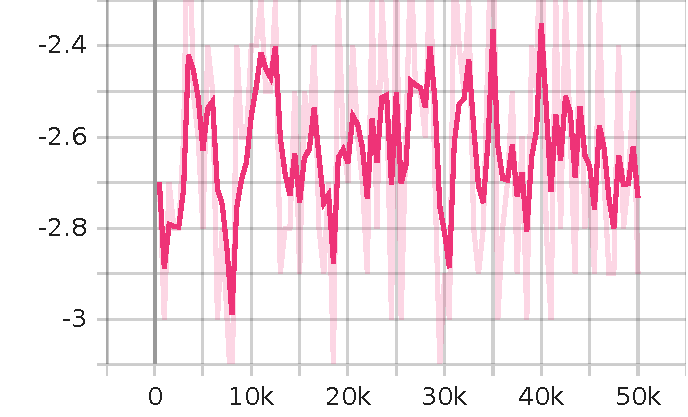
\includegraphics[scale=.6]{images/stats/ddqn_50k/Metrics_Eval_AverageReturn} }
	\caption[DDQN Training]{Metrics for the DDQN agent. In all diagrams the x-axis displays the number of training/evaluation steps. The y-axis displays the average episode number in (a) and (c), and the average return in (b) and (d).}	
	\label{fig:ddqn_train}
\end{figure}

Similarily, to the DQN (and other agents), the training and evaluation metrics, seen in figure \ref{fig:ddqn_train}, show similar values in all aspects, due to action-masking.


\section{REINFORCE}

\begin{figure}[H]
	\centering
	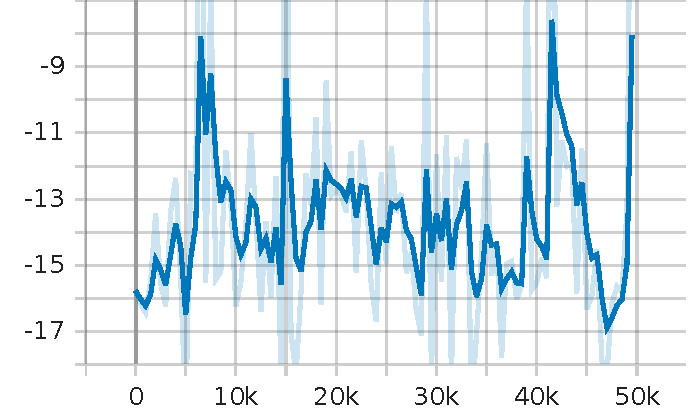
\includegraphics[scale=.75]{images/stats/reinforce_50k/Losses_policy_gradient_loss}
	\caption[REINFORCE loss]{Policy gradient loss of the REINFORCE agent in Mastermind. The x-axis displays the number of training steps and the y-axis the loss value.}
	\label{fig:reinforce_loss}
\end{figure}

In contrast to the DQN and DDQN agent, the REINFORCE agent is calculating the loss of the policy gradient, hence the difference in numbers along the x-axis. Figure \ref{fig:reinforce_loss} shows relatively high difference between the extremes, with -19.59 at 5.000 training steps being the lowest and 3.221 at 41.500 training steps the highest. However, most of the values are remaining at the same range between -11 and -16, regardless of training duration. Suggesting, that increasing training duration will not significantly improve performance.



\begin{figure}[H]
	\centering
	\subfloat[Training: Average episode length]{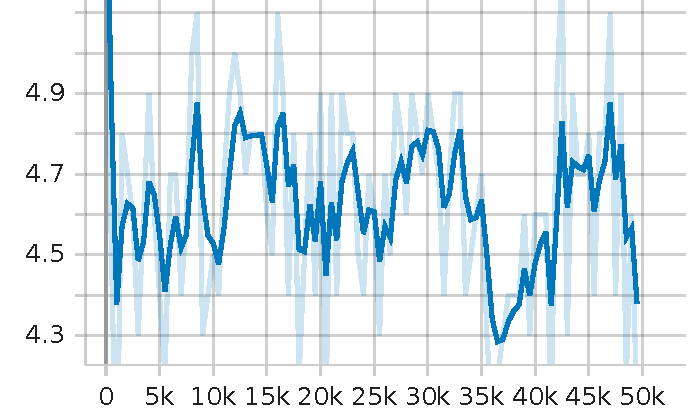
\includegraphics[scale=.6]{images/stats/reinforce_50k/Metrics_Train_AverageEpisodeLength} }
	\qquad
	\subfloat[Training: Average return]{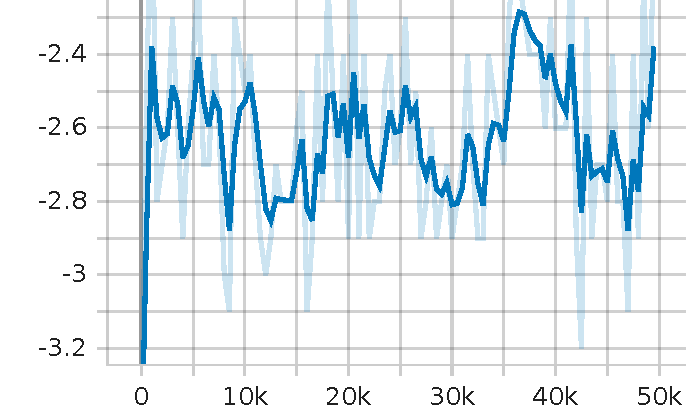
\includegraphics[scale=.6]{images/stats/reinforce_50k/Metrics_Train_AverageReturn} }
	\qquad
	\subfloat[Evaluation: Average episode length]{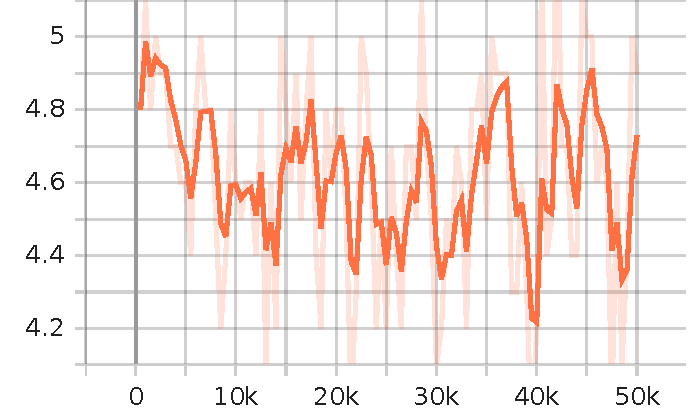
\includegraphics[scale=.6]{images/stats/reinforce_50k/Metrics_Eval_AverageEpisodeLength} }
	\qquad
	\subfloat[Evaluation: Average return]{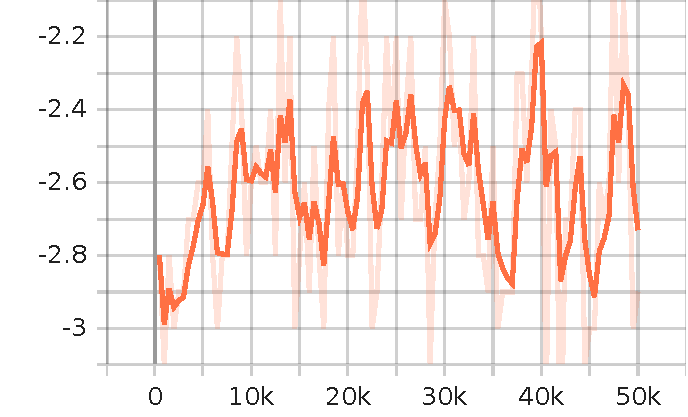
\includegraphics[scale=.6]{images/stats/reinforce_50k/Metrics_Eval_AverageReturn} }
	\caption[REINFORCE Training]{Metrics for the REINFORCE agent. In all diagrams the x-axis displays the number of training/evaluation steps. The y-axis displays the average episode number in (a) and (c), and the average return in (b) and (d).}	
	\label{fig:reinforce_train}
\end{figure}


The values of the training and evaluation metrics in figure \ref{fig:reinforce_train} indicate the same observation and are averaging the same metrics, as other agents.




\section{PPO}

\begin{figure}[H]
	\centering
	\subfloat[Policy gradient loss]{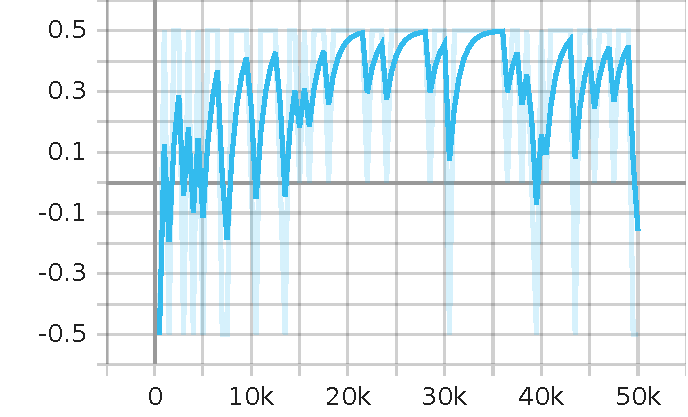
\includegraphics[scale=.6]{images/stats/ppo_50k/Losses_policy_gradient_loss} }
	\qquad
	\subfloat[Value estimation loss]{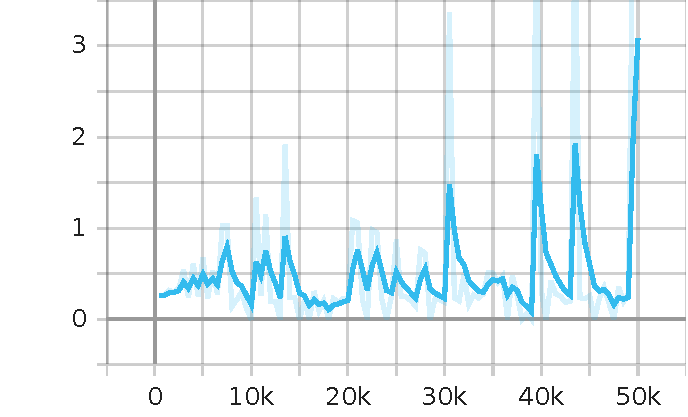
\includegraphics[scale=.6]{images/stats/ppo_50k/Losses_value_estimation_loss} }
	\caption[PPO loss]{Policy gradient loss (a) and value estimation loss (b) of the PPO agent in Mastermind. The x-axis displays the number of training steps and the y-axis the loss value.}	
	\label{fig:ppo_loss}
\end{figure}


The PPO agent has an additional loss, the value estimation loss. The policy gradient loss is constantly fluctuating between -0.5 and 0.5, as seen in figure \ref{fig:ppo_loss}. This is due to the \textit{clip} variant of the PPO method. It is by nature restricted, how far the new policy can deviate from the old one. The other loss, is from the critic of the network. Initially, the loss is relatively low, but is having increased high spikes.


\begin{figure}[H]
	\centering
	\subfloat[Training: Average episode length]{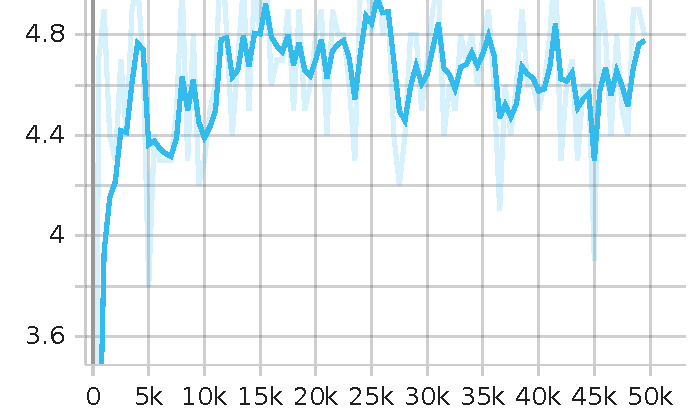
\includegraphics[scale=.6]{images/stats/ppo_50k/Metrics_Train_AverageEpisodeLength} }
	\qquad
	\subfloat[Training: Average return]{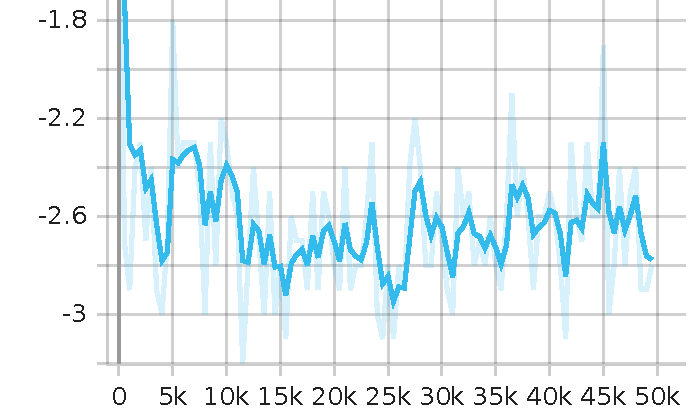
\includegraphics[scale=.6]{images/stats/ppo_50k/Metrics_Train_AverageReturn} }
	\qquad
	\subfloat[Evaluation: Average episode length]{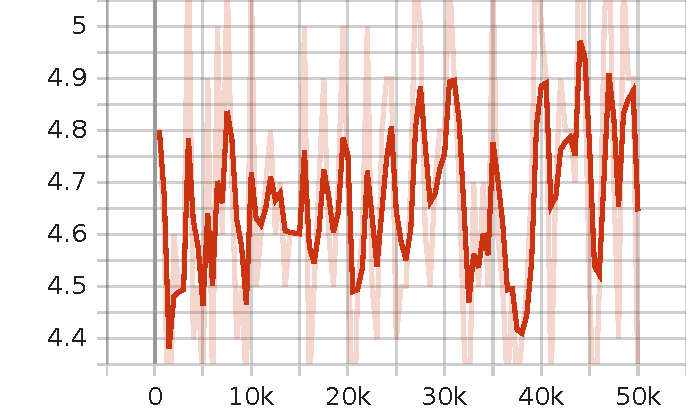
\includegraphics[scale=.6]{images/stats/ppo_50k/Metrics_Eval_AverageEpisodeLength} }
	\qquad
	\subfloat[Evaluation: Average return]{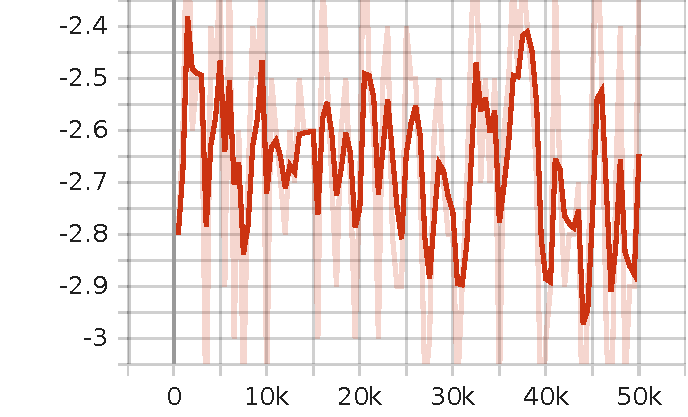
\includegraphics[scale=.6]{images/stats/ppo_50k/Metrics_Eval_AverageReturn} }
	\caption[PPO Training]{Metrics for the PPO agent. In all diagrams the x-axis displays the number of training/evaluation steps. The y-axis displays the average episode number in (a) and (c), and the average return in (b) and (d).}	
	\label{fig:ppo_train}
\end{figure}

Again, the metrics for training and evaluation show similar values as the other agents, as demonstrated in figure \ref{fig:ppo_train}.